%===============================================================================
% $Id: ifacconf.tex 19 2011-10-27 09:32:13Z jpuente $  
% Template for IFAC meeting papers
% Copyright (c) 2007-2008 International Federation of Automatic Control
%===============================================================================
\documentclass{ifacconf}
\usepackage{xcolor}

% Mude para \instrfalse para esconder todas as instruções
\newif\ifinstr \instrtrue
% \newif\ifinstr \instrfalse

\newcommand{\instr}[1]{%
  \ifinstr
    \par\noindent
    \fcolorbox{orange!80!black}{yellow!20}{%
      \parbox{\dimexpr\linewidth-2\fboxsep-2\fboxrule}{%
        \small\sffamily\color{orange!40!black}%
        \textbf{Instrução:} #1}}%
    \par\medskip
  \fi}

\newcommand{\tamanho}[1]{%
  \ifinstr
    \par\noindent
    \fcolorbox{blue!80!black}{gray!20}{%
      \parbox{\dimexpr\linewidth-2\fboxsep-2\fboxrule}{%
        \small\sffamily\color{black!40!black}%
        \textbf{Tamanho:} #1}}%
    \par\medskip
  \fi}


  
\usepackage{graphicx}      % include this line if your document contains figures
\usepackage{natbib}        % required for bibliography
%===============================================================================
\begin{document}
\begin{frontmatter}

\title{A case study for nonlinear system identification of pressure control systems\thanksref{footnoteinfo}} 
% Title, preferably not more than 10 words.

\thanks[footnoteinfo]{Sponsor and financial support acknowledgment
goes here. Paper titles should be written in uppercase and lowercase
letters, not all uppercase.}

\author[First]{Matheus Kale Mendes} 
\author[First]{Fabricio Cassanho Teodoro} 
\author[First]{Gabriel Tartari}
\author[First]{Helon Vicente Hultmann Ayala}

\address[First]{PUCPR \textbf{(completar aqui)} (e-mail: author@ boulder.nist.gov).}
% \address[First]{National Institute of Standards and Technology, Boulder, CO 80305 USA (e-mail: author@ boulder.nist.gov).}

\begin{abstract}                % Abstract of not more than 250 words.
These instructions give you guidelines for preparing papers for IFAC
technical meetings. Please use this document as a template to prepare
your manuscript. For submission guidelines, follow instructions on
paper submission system as well as the event website.

\instr{preencher apenas no final.}

\end{abstract}

\begin{keyword}
Five to ten keywords, preferably chosen from the IFAC keyword list.
\end{keyword}

\end{frontmatter}
%===============================================================================

\section{Introduction}

\tamanho{1.5 pp. (contando resumo titulo etc)}

\textit{Contextualization: } cogito ergo sum.

\instr{Contextualização: sistemas de pressão aparecem em várias aplicações
(bleed aircraft engines, processos químicos etc.). }

\textit{Motivation: } cogito ergo sum.

\instr{Justificar pq é importante. modelar e controlar pressao, simulacao é importante, data-driven simulation idem, etc.}

\textit{Literature review:}  cogito ergo sum.

\instr{Revisão da literatura: estudos de caso sobre modelagem e controle de pressão.}

\textit{Contributions:} cogito ergo sum.

\instr{Contribuição: liste em itens o que este artigo traz de novo.}

The remaining of the paper is organized as follows. In Section \ref{sec:case} ...

\section{Case Study} \label{sec:case}
\tamanho{1 p.}

\subsection{Processes Description} 

The experiment consists of pressure control in a laboratory-scale compressed-air system designed to reproduce operating conditions similar to those encountered in industrial processes.

The experimental setup comprises a compressed-air supply system driven by a screw compressor, two pressure transmitters responsible for measuring the process variables, and a proportional control valve used as the final control element.

The compressed-air pressure is regulated by modulating the opening of the proportional valve according to the control signals generated by the control system.

Pressure monitoring is performed using two transmitters installed at different locations in the experimental setup. Transmitter PT-02 measures the pressure at the system inlet, whereas PT-01 monitors the outlet pressure, which is supplied to the compressed-air consumers.

Figure \ref{fig:Esquemático Pneumatico} presents the schematic diagram of the experimental setup, highlighting the main equipment, pressure measurement points, and final control element.


\begin{figure}[!htb]
    \centering
    \caption{Process diagram of the experimental compressed-air system}
    \includegraphics[width=8.5cm]{fig/compressor.png}
    \label{fig:Esquemático Pneumatico}
    \\Source: Authors' own work
\end{figure}


\subsection{Instrumentation and Automation Description} 

The experimental setup employs a Rockwell Automation CompactLogix programmable logic controller (PLC), responsible for acquiring and processing signals from field instruments, as well as controlling the proportional valve.

The instrumentation consists of two pressure transmitters powered by a 24 V DC supply and connected to the channels of an analog input module through 4–20 mA current loops, in accordance with the analog signal standard specified in IEC 60381-1. The current signals are digitized using a 14-bit analog-to-digital converter (ADC).

Since the transmitters have different measurement ranges, namely 0–10 bar for PT-02 and 0–80 psi for PT-01, a scaling function block was implemented in the PLC to convert the acquired signals into engineering units. To ensure consistency among the pressure variables, psi was adopted as the standard pressure unit throughout the control system.

The proportional valve is actuated by the PLC through an analog output module that generates a 4–20 mA current signal. This signal is produced by a 14-bit digital-to-analog converter (DAC), which converts the control command, expressed as a percentage of valve opening, into a current signal proportional to the valve operating range, as illustrated in Fig. \ref{fig:Esquemático elétrico}.

\begin{figure}[!htb]
    \centering
    \caption{Instrumentation diagram}
    \includegraphics[width=8.5cm]{fig/Instrumentacao.png}
    \label{fig:Esquemático elétrico}
    \\Source: Authors' own work
\end{figure}

The process signals are made available through a human–machine interface (HMI) developed using the Elipse E3 platform, which provides supervisory control, process monitoring, and operational data logging. Communication between the CompactLogix PLC and the supervisory system is established using the Common Industrial Protocol (CIP) over the EtherNet/IP industrial communication network, as illustrated in Fig. \ref{fig:Esquemático automação}.

\begin{figure}[!htb]
	\centering
	\caption{Diagrama de automação}
	\includegraphics[width=8.5cm]{fig/IHM.png}
    \label{fig:Esquemático automação}
	\\Fonte: Authors' own work
\end{figure}

\section{Experimental Design} \label{sec:exp_design}
\tamanho{1 p.}

\instr{Describe excitation signals (plot them on a graph)}

\instr{Describe measured output signals (plot them on a graph).}

\subsection{Preliminary Nonlinear Characterization} \label{subsec:quasi_static}

Before designing the dynamic excitation signal for system identification, a preliminary quasi-static ramp test (\texttt{Quasi\_Static\_Test}, Fig.~\ref{fig:quasi_static}) was conducted on the experimental bench to investigate the nonlinear behavior of the pneumatic plant \citep{Schwarz2024ModelBased,Wehmeier2026HydraulicPoppet}. In this test (sampled at $1~\text{Hz}$ over $17.1~\text{minutes}$), the proportional valve was initially kept closed ($\mathrm{CV} = 0\%$), driven through a slow linear opening ramp from $0\%$ to $100\%$ over $3~\text{minutes}$, held fully open at $100\%$ for $5~\text{minutes}$, and subsequently closed linearly from $100\%$ back to $0\%$ over $3~\text{minutes}$, remaining closed until the system settled.

\begin{figure}[!ht]
\begin{center}
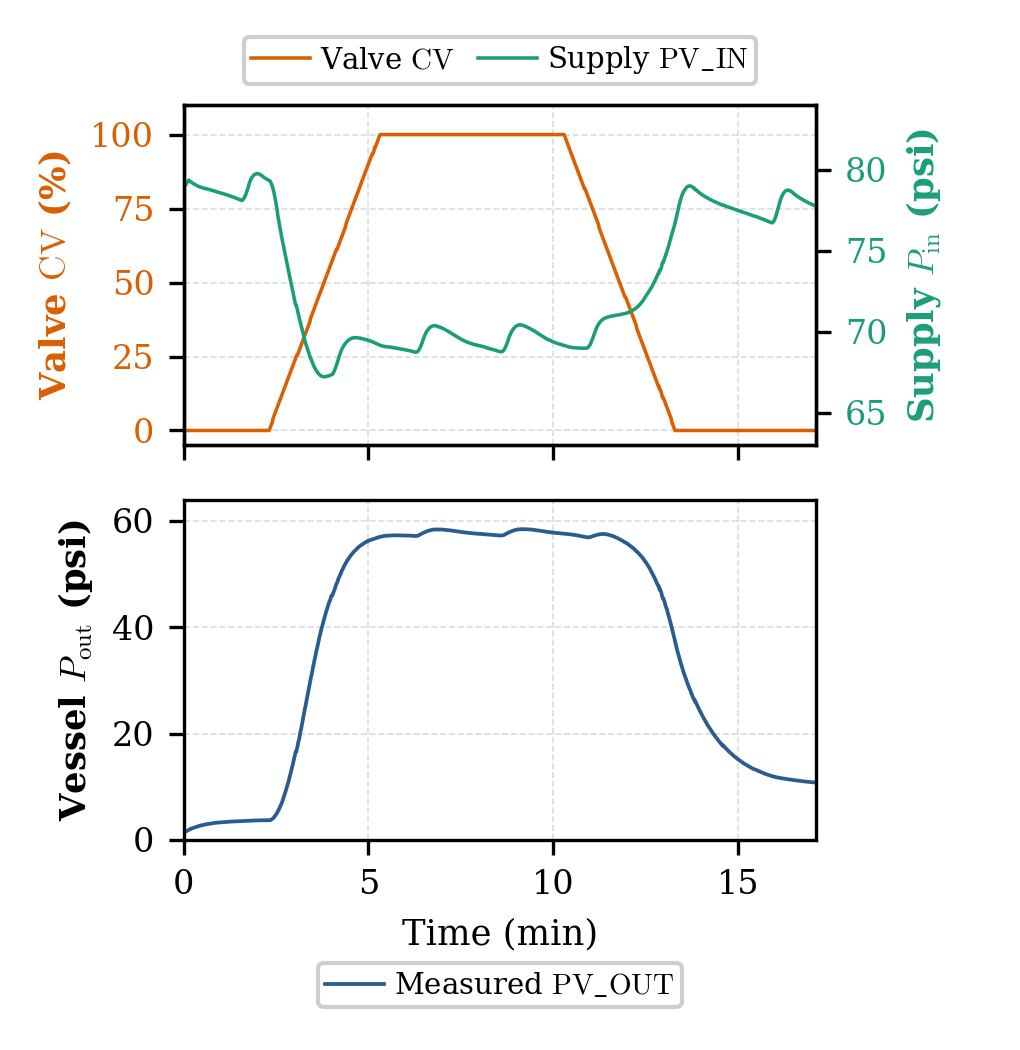
\includegraphics[width=8.4cm]{fig/Quasi_Static_Test.png}
\caption{Preliminary quasi-static ramp test (\texttt{Quasi\_Static\_Test}): proportional valve command ($\mathrm{CV}$) and filtered supply pressure ($\mathrm{PV\_IN}$) in the top panel; nonlinear downstream pressure response ($\mathrm{PV\_OUT}$) in the bottom panel.} 
\label{fig:quasi_static}
\end{center}
\end{figure}

The experimental response in Fig.~\ref{fig:quasi_static} reveals three fundamental nonlinear phenomena that motivate a MISO nonlinear modeling approach:
\begin{enumerate}
    \item \textbf{Valve orifice flow saturation:} During the rising ramp, the outlet pressure ($\mathrm{PV\_OUT}$) increases steeply for $\mathrm{CV}$ between $10\%$ and $65\%$, but saturates around $57\text{--}58~\text{psi}$ once the opening exceeds $\mathrm{CV} \approx 70\%$, demonstrating that the static gain varies strongly across the operating range \citep{Schwarz2024ModelBased}.
    \item \textbf{Upstream supply pressure coupling ($\mathrm{PV\_IN}$):} As the valve opens and air consumption increases, the filtered upstream supply pressure drops from approximately $79~\text{psi}$ to $68\text{--}70~\text{psi}$, oscillating with the compressor regulation cycles and directly modulating the maximum pressure plateau reached by $\mathrm{PV\_OUT}$.
    \item \textbf{Hysteresis and charging/discharging asymmetry:} During the falling ramp ($t = 10.3$ to $13.3~\text{min}$), $\mathrm{PV\_OUT}$ remains nearly unchanged as the valve closes from $100\%$ down to $70\%$ and, after full closure at $t = 13.3~\text{min}$, exhibits a slow exponential depressurization tail that takes over $3.5~\text{minutes}$ to decay toward $11~\text{psi}$ \citep{Sun2025PneumaticSoftActuator}.
\end{enumerate}

\subsection{Excitation Signal Design and Measured Process Signals} \label{subsec:measured_signals}

To properly excite both static and dynamic nonlinearities across the entire operating envelope, an open-loop excitation signal was synthesized in MATLAB (\texttt{generate\_excitation\_signals.m}) at the same sampling rate as the Elipse E3 supervisory system ($f_s = 4~\text{Hz}$, $T_s = 0.25~\text{s}$) and exported in CSV format for direct execution by the automation system. Among the three test profiles available in the repository---quasi-static ramp, random steps (\textit{Random Steps}), and frequency-swept sine (\textit{Swept-Sine / Chirp})---the \textbf{Random Steps} sequence was selected for dynamic system identification \citep{Lee2025EnergyReduction}. Generated with a fixed pseudo-random seed (\texttt{rng(0)}) for reproducibility, the excitation consists of $60$ consecutive plateaus of constant duration $T_{\text{step}} = 60~\text{s}$ ($240$ samples per step), with proportional valve opening amplitudes ($\mathrm{CV}$) drawn uniformly between $0\%$ and $100\%$. The $60~\text{s}$ dwell time per plateau was chosen to exceed the dominant plant time constant ($\tau \approx 28~\text{s}$), capturing both transient transitions and steady-state settling across multiple pressure levels, with initial and final rest intervals at $\mathrm{CV} = 0\%$.

Fig.~\ref{fig:acquisition_data} presents both the applied excitation profile and the resulting process response acquired on the bench during the \texttt{Random Steps\_4.csv} assay, totaling $64.4~\text{minutes}$ of continuous operation ($15,466$ samples at $4~\text{Hz}$). Combining the excitation and response into a single figure directly illustrates the input--output causality: the top panel shows the proportional valve opening command ($\mathrm{CV}$), while the bottom panel displays the measured downstream vessel pressure ($\mathrm{PV\_OUT}$), which is used in its entirety ($100\%$ training dataset) for model identification.

\begin{figure}[!ht]
\begin{center}
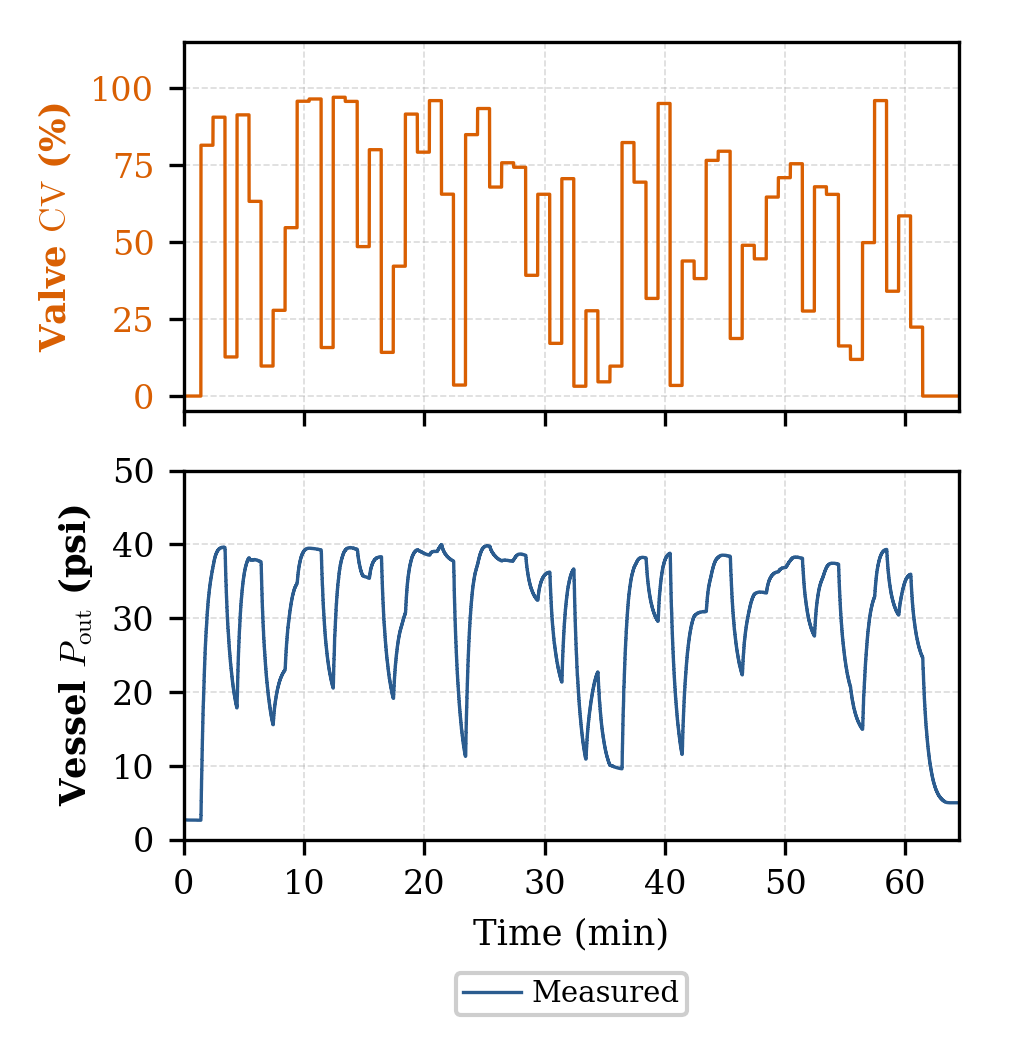
\includegraphics[width=8.4cm]{fig/acquisition_data.png}
\caption{Experimental identification dataset (\texttt{Random Steps\_4}): applied random-step proportional valve excitation command ($\mathrm{CV}$) in the top panel; measured downstream vessel pressure response ($\mathrm{PV\_OUT}$, 100\% identification training dataset) in the bottom panel.} 
\label{fig:acquisition_data}
\end{center}
\end{figure}

Analysis of the experimental data in Fig.~\ref{fig:acquisition_data} highlights three key features for system identification:
\begin{enumerate}
    \item \textbf{Upstream supply pressure behavior ($\mathrm{PV\_IN}$):} Although omitted from Fig.~\ref{fig:acquisition_data} for visual clarity, the filtered upstream supply pressure measured by PT-02 is logged concurrently throughout the $64.4\text{-minute}$ assay, oscillating between approximately $60~\text{psi}$ and $80~\text{psi}$ due to the screw compressor on--off regulation band and air draw during filling, and is incorporated directly as the second exogenous input in the MISO model.
    \item \textbf{Operating range and variable gain of the output ($\mathrm{PV\_OUT}$):} The receiver tank pressure responds to the valve steps across a wide range from $2.8~\text{psi}$ to $40.0~\text{psi}$. Steps of equal amplitude in $\mathrm{CV}$ produce different pressure variations depending on the operating point and the instantaneous supply pressure ($\mathrm{PV\_IN}$).
    \item \textbf{Dynamic asymmetry across multiple plateaus:} Throughout the entire assay, rapid rising transitions are observed during pressurization, followed by slow, nonlinear decay curves whenever the valve opening is reduced.
\end{enumerate}

\subsection{Access to the datasets} \label{subsec:datasets}

\instr{Create a github repo; check the guidelines of Scientific Data, for example; check the BAB datasets)}

Despite growing interest in data-driven modeling and digital twins for pneumatic and fluid power systems, publicly available experimental datasets acquired from real industrial instrumentation remain scarce in the literature \citep{Khamkar2024DigitalTwinFluidPower,Pawluchin2026DataDriven}. To provide an open and reproducible benchmark for the system identification and control community, all experimental datasets, MATLAB excitation generation scripts, and Python ARX/NARX identification routines have been made publicly available in the GitHub repository: \texttt{https://github.com/Matheus2091/pressure-plant-case-study}. Following scientific data-sharing best practices, the files are provided in open tabular format (\texttt{.csv}) with standardized headers (\texttt{Timestamp}, \texttt{CV}, \texttt{PV\_OUT}, and \texttt{PV\_IN}) alongside documentation of the CompactLogix PLC and Elipse E3 supervisory architecture.

The datasets will continue to evolve as more acquisitions are made available, as the repository will allow to download more up to date datasets. The repository will be tagged so the comparisons will be readily available according to a given dataset recquired. 

\section{Results} \label{sec:results}
\tamanho{1.5 pp.}

In this section, we present and evaluate a data-driven black-box identification framework for the pneumatic pressure control plant using the sensory information described in Section~\ref{sec:case}. First, we establish the model creation setup, including variable definitions, regressor search spaces, structure selection via Orthogonal Least Squares (OLS), and validation criteria. Next, we report the identification and time-domain validation of a linear baseline MISO ARX (AutoRegressive with eXogenous inputs) model. We then detail the identification of a nonlinear polynomial MISO NARX model, providing a physical interpretation of the terms selected by the algorithm. Finally, we present a quantitative error comparison between both models under one-step-ahead (OSA) prediction and recursive open-loop free-run (FR) simulation, discussing how the resulting model enables soft sensing and simulation for control design.

\instr{adicionar no paragrafo acima um resumo do que se encontra na secao}

\subsection{Identification Setup and Validation Protocol} \label{subsec:setup}

To capture the plant dynamics, a MISO (Multiple-Input Single-Output) identification architecture was formulated by mapping the instrumentation signals from Section~\ref{sec:case} into a discrete-time input--output representation. Specifically, the model output $y(k)$ corresponds to the regulated downstream outlet pressure measured by transmitter PT-01 ($\mathrm{PV\_OUT}$), whereas the two exogenous inputs comprise the proportional control valve command $u_1(k) = \mathrm{CV}(k)$ and the filtered upstream supply header pressure $u_2(k) = \mathrm{PV\_IN}(k)$ measured by inlet transmitter PT-02. Including $\mathrm{PV\_IN}(k)$ as a second exogenous input is essential because the screw compressor operates under an on--off control band and air is drawn from the supply line during filling, causing inlet pressure fluctuations that directly affect the mass flow rate across the valve.

The experimental identification protocol and hyperparameter configuration are summarized as follows:
\begin{itemize}
    \item \textbf{Dataset and sampling:} The experimental run (\texttt{Random Steps\_4.csv}, described in Section~\ref{subsec:measured_signals} and illustrated in Fig.~\ref{fig:acquisition_data}) consists of random step excitations applied to the proportional valve over $64.4~\text{minutes}$ of operation, sampled at $f_s = 4~\text{Hz}$ ($\Delta t = 0.25~\text{s}$), totaling $N = 15,466$ samples.
    
    \item \textbf{Unified identification dataset:} The entire $64.4~\text{minutes}$ ($15,466$ samples) of the open-loop assay is utilized as the identification dataset for structure selection and parameter estimation, maximizing data diversity across all operating regimes. Independent validation is conducted through recursive multi-step simulation and closed-loop control assays.
    
    \item \textbf{MISO variables:} System output $y(k) = \mathrm{PV\_OUT}(k)$ [psi] (downstream outlet pressure at PT-01); control input $u_1(k) = \mathrm{CV}(k)$ [\%] (valve opening command); and exogenous disturbance input $u_2(k) = \mathrm{PV\_IN}(k)$ [psi] (filtered upstream supply pressure at PT-02).
    
    \item \textbf{Lag orders and candidate search space:} Equal maximum lags of $n_y = 3$, $n_{u_1} = 3$, and $n_{u_2} = 3$ (spanning $0.75~\text{s}$ of past history, or $9$ base lagged regressors) are adopted for both models. The linear MISO ARX model uses polynomial degree $\ell = 1$ ($10$ candidate regressors including the constant term, with $6$ terms retained), whereas the MISO NARX model expands the basis up to cubic degree $\ell = 3$, generating $\binom{9+3}{3} = 220$ candidate monomials from which $8$ terms are selected.
    
    \item \textbf{Structure selection algorithm:} Structure selection and parameter estimation are performed via Orthogonal Least Squares (OLS for ARX and FROLS for NARX), ranking candidate regressors greedily according to the Error Reduction Ratio (ERR) criterion \citep{Chen1989Orthogonal,Billings2013Nonlinear}.
    
    \item \textbf{Validation regimes and performance metric:} Model accuracy is assessed under both One-Step-Ahead (OSA) prediction, where measured past outputs $y(k-i)$ are fed back at each step, and open-loop Free-Run (FR) simulation, where the model is initialized only with the first $n_y = 3$ samples and predicts across the entire $15,463$-step horizon using its own recursive past estimates $\hat{y}_{\mathrm{FR}}(k-i)$ alongside the measured inputs $\mathrm{CV}$ and $\mathrm{PV\_IN}$. Prediction accuracy is quantified by the Root Mean Squared Error (RMSE), expressed in psi:
    \begin{equation}
        \mathrm{RMSE} = \sqrt{\frac{1}{N - n_y} \sum_{k = n_y + 1}^{N} \left( y(k) - \hat{y}(k) \right)^2} \, .
        \label{eq:rmse}
    \end{equation}
\end{itemize}

\instr{Descrever todas as condições para criar os modelos (hiperparametros). Definir protocolo de treino e teste (quais datasets sao usados e para que, referenciar secao anterior). Metrica para comparacao (RMSE). \textbf{2A FEIRA}}

\subsection{Linear MISO ARX Modeling} \label{subsec:arx}

\instr{Resultados ARX modeling (linear model). Modelo final, plot dado vs. teste (FR). \textbf{Começar com figuras / bullets} \textbf{2A FEIRA}}

To establish a baseline, the MISO ARX structure was identified from the dynamic dataset. Fig.~\ref{fig:arx_results} compares the measured downstream pressure against the linear ARX model responses in OSA prediction and open-loop Free-Run simulation. The resulting difference equation with the $6$ regressors selected via ERR is given by:
\begin{equation}
\begin{array}{rl}
y(k) = & 0.991\,y(k-1) \\
       & + 2.13\times 10^{-3}\,\mathrm{CV}(k-1) \\
       & - 0.093\,\mathrm{PV\_IN}(k-1) \\
       & + 0.207\,\mathrm{PV\_IN}(k-2) \\
       & - 0.122\,\mathrm{PV\_IN}(k-3) \\
       & + 0.772 \, .
\end{array}
\label{eq:arx_model}
\end{equation}

A detailed examination of the linear ARX identification yields the following findings:
\begin{itemize}
    \item \textbf{Dominant autoregressive regressor:} The first-order lagged output $y(k-1)$ accounts for $\mathrm{ERR} = 99.998\%$ of the output variance, reflecting a slow dominant discrete-time pole at $z = 0.991$ (corresponding to an effective time constant of $\tau \approx 27.9~\text{s}$). The remaining five linear terms provide constant-gain input corrections.
    \item \textbf{Discrepancy between OSA and Free-Run accuracy:} On the complete dataset, the ARX model achieves an OSA RMSE of $0.122~\text{psi}$. However, when operated recursively in open-loop simulation without output feedback, the Free-Run RMSE rises to $2.320~\text{psi}$.
    \item \textbf{Structural limitation of linear dynamics:} As evidenced in the bottom panel of Fig.~\ref{fig:arx_results}, the linear Free-Run trajectory exhibits systematic overshoot during large pressure transitions and noticeable drift during low-pressure discharge intervals. Because a linear ARX model enforces a fixed pole and constant input gains across all operating points, it fails to capture the asymmetric charging/discharging rates and pressure-dependent flow gains inherent to compressible gas systems.
\end{itemize}

\begin{figure}[!ht]
\begin{center}
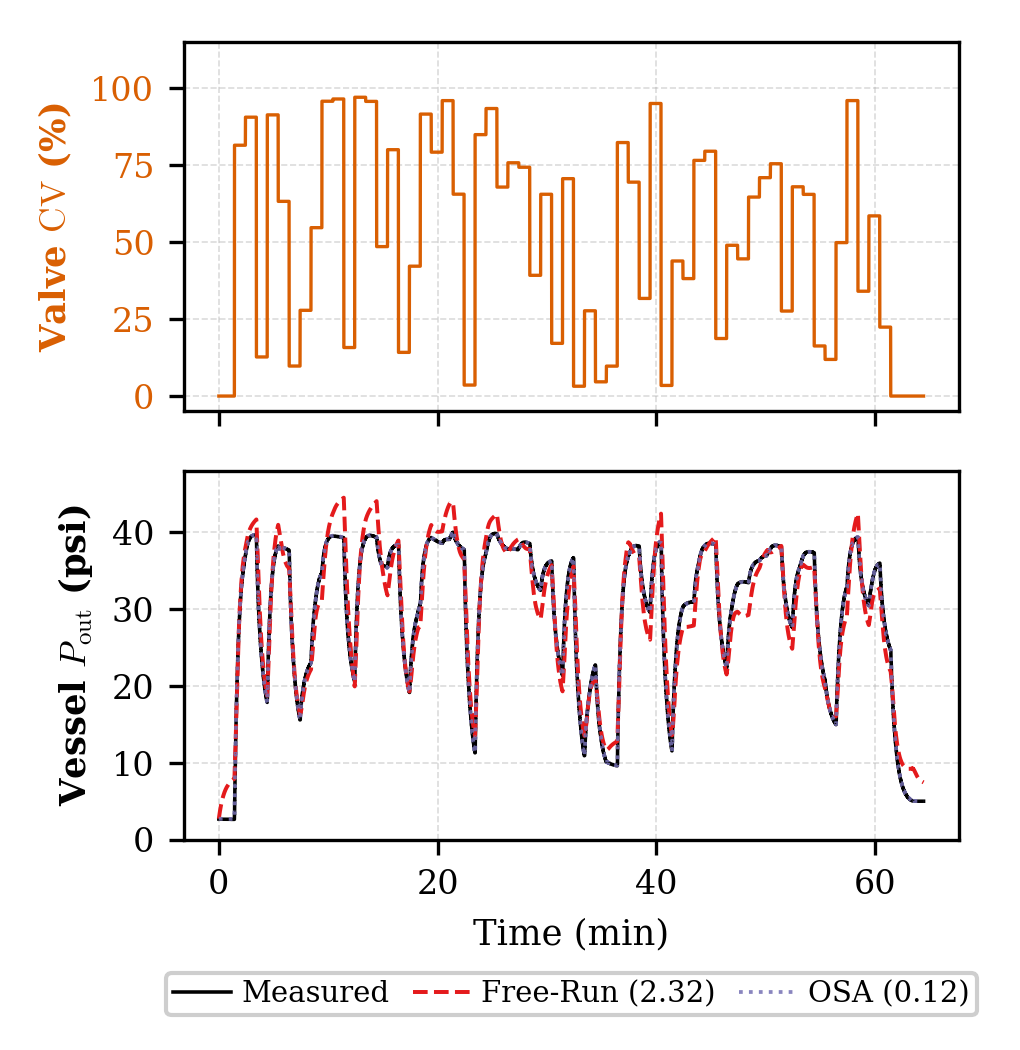
\includegraphics[width=7.7cm]{fig/Resultado_ARX_1.png}
\caption{Linear ARX model evaluation on the identification dataset: applied valve opening command $\mathrm{CV}$ in the top panel; open-loop simulation (Free-Run) and one-step-ahead prediction (OSA) compared against measured pressure in the bottom panel.} 
\label{fig:arx_results}
\end{center}
\end{figure}

\subsection{Nonlinear Polynomial MISO NARX Modeling} \label{subsec:narx}

\instr{Resultados NARX modeling (nonlinear model).\textbf{ Começar com figuras / bullets} \textbf{2A FEIRA}}

To overcome the limitations of the linear baseline, the polynomial MISO NARX model was identified from the $220$-term candidate dictionary using the FROLS algorithm, retaining $8$ terms that together explain $99.999\%$ of the output variance. The identified MISO NARX model equation is expressed as:
\begin{equation}
\begin{array}{rl}
y(k) = & 0.548\,y(k-1) + 0.445\,y(k-3) \\
       & + 8.29\times 10^{-3}\,\mathrm{CV}(k-3) \\
       & + 8.37\times 10^{-7}\,\mathrm{CV}(k-1)\mathrm{PV\_IN}^2(k-2) \\
       & - 6.66\times 10^{-7}\,y(k-1)\mathrm{CV}^2(k-1) \\
       & - 1.86\times 10^{-4}\,y^2(k-3)\mathrm{PV\_IN}(k-1) \\
       & + 1.84\times 10^{-4}\,y^2(k-3)\mathrm{PV\_IN}(k-2) \\
       & - 3.84\times 10^{-5}\,\mathrm{CV}^2(k-3) \, .
\end{array}
\label{eq:narx_model}
\end{equation}

Fig.~\ref{fig:narx_results} illustrates the time-domain performance of the MISO NARX model under both OSA and Free-Run regimes. Key insights from the NARX identification include:
\begin{itemize}
    \item \textbf{Physical interpretation of FROLS-selected terms:} Beyond the linear autoregressive terms $y(k-1)$ ($\mathrm{ERR} = 99.998\%$) and $y(k-3)$ and the linear valve term $\mathrm{CV}(k-3)$, the FROLS algorithm selected five cubic cross-coupling monomials that mirror the governing physics of pneumatic systems \citep{Du2024ReviewDigitalPneumatic}. In particular, the term $\mathrm{CV}(k-1)\mathrm{PV\_IN}^2(k-2)$ captures the nonlinear scaling of mass flow with supply pressure and valve opening. The state--input product $-6.66\times 10^{-7}\,y(k-1)\mathrm{CV}^2(k-1)$ modulates the effective system pole with the valve position, capturing the physical reduction in the pneumatic time constant when the valve is widely open. Furthermore, the quadratic valve term $-3.84\times 10^{-5}\,\mathrm{CV}^2(k-3)$ represents orifice flow saturation at large openings, and the paired terms $\mp 1.85\times 10^{-4}\,y^2(k-3)\mathrm{PV\_IN}$ account for pressure-dependent chamber compressibility.
    \item \textbf{Substantial Free-Run error reduction:} In open-loop Free-Run simulation, the NARX model achieves an RMSE of $0.813~\text{psi}$, cutting the simulation error by $65.0\%$ compared to the linear ARX model ($2.320~\text{psi}$), while the OSA RMSE drops to $0.101~\text{psi}$ (a $17.2\%$ improvement).
    \item \textbf{Long-horizon trajectory tracking:} As shown in Fig.~\ref{fig:narx_results}, the NARX Free-Run simulation tightly tracks the measured downstream pressure across all $15,463$ steps without accumulating drift, faithfully capturing both sharp pressurization steps up to $40~\text{psi}$ and prolonged nonlinear depressurization tails down to $5~\text{psi}$.
\end{itemize}

\begin{figure}[!ht]
\begin{center}
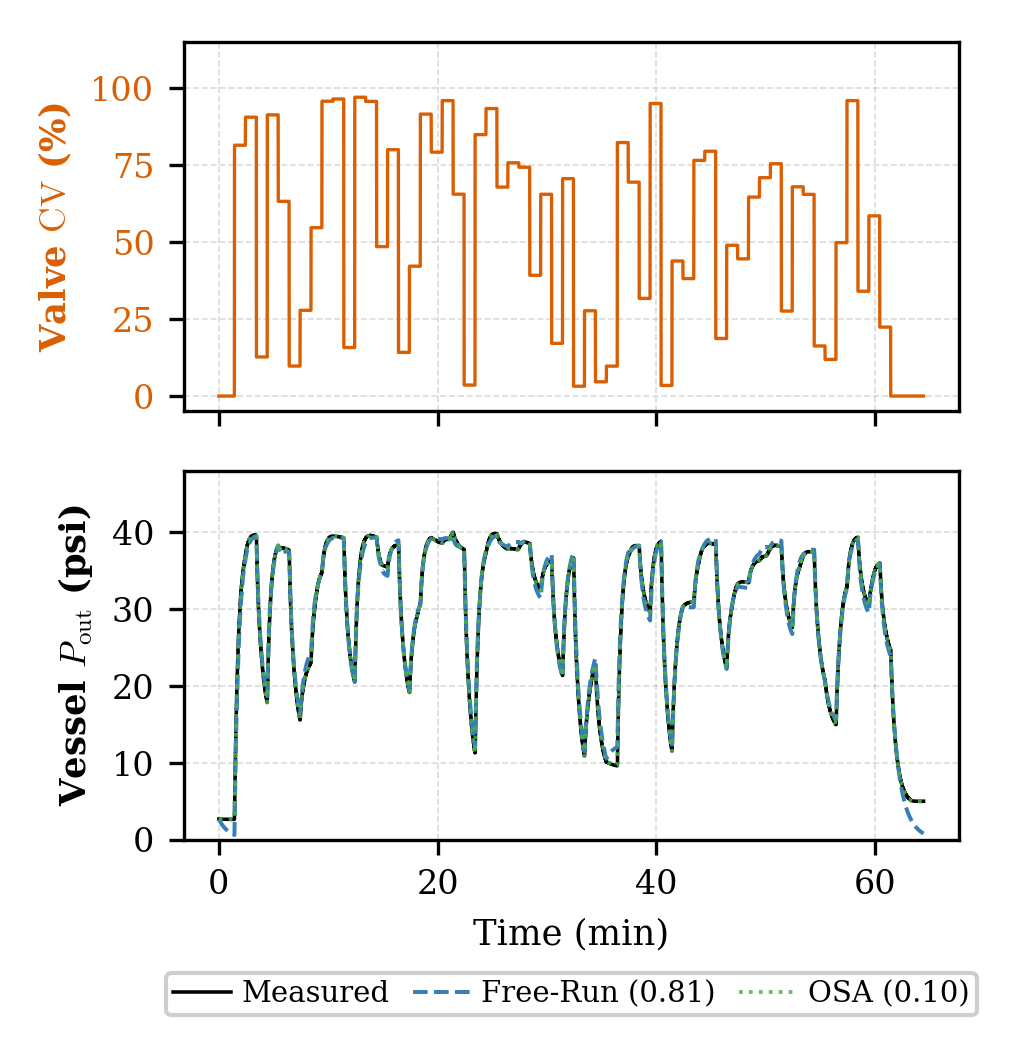
\includegraphics[width=7.7cm]{fig/Resultados_NARX_1.png}
\caption{Nonlinear NARX model evaluation on the identification dataset: applied valve opening command $\mathrm{CV}$ in the top panel; open-loop simulation (Free-Run) and OSA prediction compared against measured pressure in the bottom panel.} 
\label{fig:narx_results}
\end{center}
\end{figure}

\subsection{Comparative Analysis and Model Application} \label{subsec:comparison}

\instr{Tabela comparativa (RMSE).}

\begin{table}[!ht]
\begin{center}
\caption{Performance comparison between ARX and NARX models on the identification dataset (RMSE in psi).}\label{tb:comparison}
\begin{tabular}{lcc}
\hline
Model & One-Step-Ahead (OSA) & Free-Run (FR) \\ \hline
ARX (Linear, $\ell=1$, 6 terms)     & 0.122 & 2.320 \\
NARX (Nonlinear, $\ell=3$, 8 terms) & \textbf{0.101} & \textbf{0.813} \\ \hline
Relative Improvement (\%)           & 17.2\% & \textbf{65.0\%} \\ \hline
\end{tabular}
\end{center}
\end{table}

\instr{Soft sensing (1st model the sensor according to the command and output pressure and 2nd use it for simulation -- with simulation data only from the model)}

Table~\ref{tb:comparison} consolidates the quantitative performance of the identified ARX and NARX models across both prediction and recursive simulation regimes. A critical methodological observation arises from comparing the OSA and FR metrics: because the sampling period ($\Delta t = 0.25~\text{s}$) is small compared to the dominant pneumatic time constant ($\tau \approx 28~\text{s}$), consecutive pressure measurements satisfy $y(k) \approx y(k-1)$, allowing even a purely linear model to achieve a low OSA RMSE of $0.122~\text{psi}$. Consequently, single-step metrics alone fail to expose structural model deficiencies. Only under open-loop Free-Run simulation---where single-step errors accumulate recursively over more than $15,000$ steps without state reset---does the superiority of the NARX representation become evident, reducing the simulation error by $65.0\%$ with just two additional parameters ($8$ vs.\ $6$ terms) \citep{Billings2013Nonlinear}.

Furthermore, the ability of the identified NARX model to operate in open-loop Free-Run mode using only the valve command $\mathrm{CV}(k)$ and upstream supply pressure $\mathrm{PV\_IN}(k)$ allows it to serve both as a virtual sensor (soft sensor) and as an accurate plant simulator \citep{Khamkar2024DigitalTwinFluidPower}. This capability enables offline design, linearization, and tuning of closed-loop controllers (such as PI controllers) directly in simulation prior to experimental deployment on the plant PLC \citep{Liu2025GAHOFOPID}.

\section{Conclusion}

\tamanho{1 p. (contando as referências)}

The present paper proposed a new case study on pressure modeling ... 

\begin{ack}
Place acknowledgments here.
\end{ack}

\bibliography{ifacconf}      

\end{document}
